% Options for packages loaded elsewhere
\PassOptionsToPackage{unicode}{hyperref}
\PassOptionsToPackage{hyphens}{url}
%
\documentclass[
  man,floatsintext]{apa7}
\usepackage{amsmath,amssymb}
\usepackage{lmodern}
\usepackage{iftex}
\ifPDFTeX
  \usepackage[T1]{fontenc}
  \usepackage[utf8]{inputenc}
  \usepackage{textcomp} % provide euro and other symbols
\else % if luatex or xetex
  \usepackage{unicode-math}
  \defaultfontfeatures{Scale=MatchLowercase}
  \defaultfontfeatures[\rmfamily]{Ligatures=TeX,Scale=1}
\fi
% Use upquote if available, for straight quotes in verbatim environments
\IfFileExists{upquote.sty}{\usepackage{upquote}}{}
\IfFileExists{microtype.sty}{% use microtype if available
  \usepackage[]{microtype}
  \UseMicrotypeSet[protrusion]{basicmath} % disable protrusion for tt fonts
}{}
\makeatletter
\@ifundefined{KOMAClassName}{% if non-KOMA class
  \IfFileExists{parskip.sty}{%
    \usepackage{parskip}
  }{% else
    \setlength{\parindent}{0pt}
    \setlength{\parskip}{6pt plus 2pt minus 1pt}}
}{% if KOMA class
  \KOMAoptions{parskip=half}}
\makeatother
\usepackage{xcolor}
\usepackage{graphicx}
\makeatletter
\def\maxwidth{\ifdim\Gin@nat@width>\linewidth\linewidth\else\Gin@nat@width\fi}
\def\maxheight{\ifdim\Gin@nat@height>\textheight\textheight\else\Gin@nat@height\fi}
\makeatother
% Scale images if necessary, so that they will not overflow the page
% margins by default, and it is still possible to overwrite the defaults
% using explicit options in \includegraphics[width, height, ...]{}
\setkeys{Gin}{width=\maxwidth,height=\maxheight,keepaspectratio}
% Set default figure placement to htbp
\makeatletter
\def\fps@figure{htbp}
\makeatother
\setlength{\emergencystretch}{3em} % prevent overfull lines
\providecommand{\tightlist}{%
  \setlength{\itemsep}{0pt}\setlength{\parskip}{0pt}}
\setcounter{secnumdepth}{-\maxdimen} % remove section numbering
% Make \paragraph and \subparagraph free-standing
\ifx\paragraph\undefined\else
  \let\oldparagraph\paragraph
  \renewcommand{\paragraph}[1]{\oldparagraph{#1}\mbox{}}
\fi
\ifx\subparagraph\undefined\else
  \let\oldsubparagraph\subparagraph
  \renewcommand{\subparagraph}[1]{\oldsubparagraph{#1}\mbox{}}
\fi
\newlength{\cslhangindent}
\setlength{\cslhangindent}{1.5em}
\newlength{\csllabelwidth}
\setlength{\csllabelwidth}{3em}
\newlength{\cslentryspacingunit} % times entry-spacing
\setlength{\cslentryspacingunit}{\parskip}
\newenvironment{CSLReferences}[2] % #1 hanging-ident, #2 entry spacing
 {% don't indent paragraphs
  \setlength{\parindent}{0pt}
  % turn on hanging indent if param 1 is 1
  \ifodd #1
  \let\oldpar\par
  \def\par{\hangindent=\cslhangindent\oldpar}
  \fi
  % set entry spacing
  \setlength{\parskip}{#2\cslentryspacingunit}
 }%
 {}
\usepackage{calc}
\newcommand{\CSLBlock}[1]{#1\hfill\break}
\newcommand{\CSLLeftMargin}[1]{\parbox[t]{\csllabelwidth}{#1}}
\newcommand{\CSLRightInline}[1]{\parbox[t]{\linewidth - \csllabelwidth}{#1}\break}
\newcommand{\CSLIndent}[1]{\hspace{\cslhangindent}#1}
\ifLuaTeX
\usepackage[bidi=basic]{babel}
\else
\usepackage[bidi=default]{babel}
\fi
\babelprovide[main,import]{english}
% get rid of language-specific shorthands (see #6817):
\let\LanguageShortHands\languageshorthands
\def\languageshorthands#1{}
% Manuscript styling
\usepackage{upgreek}
\captionsetup{font=singlespacing,justification=justified}

% Table formatting
\usepackage{longtable}
\usepackage{lscape}
% \usepackage[counterclockwise]{rotating}   % Landscape page setup for large tables
\usepackage{multirow}		% Table styling
\usepackage{tabularx}		% Control Column width
\usepackage[flushleft]{threeparttable}	% Allows for three part tables with a specified notes section
\usepackage{threeparttablex}            % Lets threeparttable work with longtable

% Create new environments so endfloat can handle them
% \newenvironment{ltable}
%   {\begin{landscape}\centering\begin{threeparttable}}
%   {\end{threeparttable}\end{landscape}}
\newenvironment{lltable}{\begin{landscape}\centering\begin{ThreePartTable}}{\end{ThreePartTable}\end{landscape}}

% Enables adjusting longtable caption width to table width
% Solution found at http://golatex.de/longtable-mit-caption-so-breit-wie-die-tabelle-t15767.html
\makeatletter
\newcommand\LastLTentrywidth{1em}
\newlength\longtablewidth
\setlength{\longtablewidth}{1in}
\newcommand{\getlongtablewidth}{\begingroup \ifcsname LT@\roman{LT@tables}\endcsname \global\longtablewidth=0pt \renewcommand{\LT@entry}[2]{\global\advance\longtablewidth by ##2\relax\gdef\LastLTentrywidth{##2}}\@nameuse{LT@\roman{LT@tables}} \fi \endgroup}

% \setlength{\parindent}{0.5in}
% \setlength{\parskip}{0pt plus 0pt minus 0pt}

% Overwrite redefinition of paragraph and subparagraph by the default LaTeX template
% See https://github.com/crsh/papaja/issues/292
\makeatletter
\renewcommand{\paragraph}{\@startsection{paragraph}{4}{\parindent}%
  {0\baselineskip \@plus 0.2ex \@minus 0.2ex}%
  {-1em}%
  {\normalfont\normalsize\bfseries\itshape\typesectitle}}

\renewcommand{\subparagraph}[1]{\@startsection{subparagraph}{5}{1em}%
  {0\baselineskip \@plus 0.2ex \@minus 0.2ex}%
  {-\z@\relax}%
  {\normalfont\normalsize\itshape\hspace{\parindent}{#1}\textit{\addperi}}{\relax}}
\makeatother

% \usepackage{etoolbox}
\makeatletter
\patchcmd{\HyOrg@maketitle}
  {\section{\normalfont\normalsize\abstractname}}
  {\section*{\normalfont\normalsize\abstractname}}
  {}{\typeout{Failed to patch abstract.}}
\patchcmd{\HyOrg@maketitle}
  {\section{\protect\normalfont{\@title}}}
  {\section*{\protect\normalfont{\@title}}}
  {}{\typeout{Failed to patch title.}}
\makeatother

\usepackage{xpatch}
\makeatletter
\xapptocmd\appendix
  {\xapptocmd\section
    {\addcontentsline{toc}{section}{\appendixname\ifoneappendix\else~\theappendix\fi\\: #1}}
    {}{\InnerPatchFailed}%
  }
{}{\PatchFailed}
\keywords{keywords\newline\indent Word count: X}
\DeclareDelayedFloatFlavor{ThreePartTable}{table}
\DeclareDelayedFloatFlavor{lltable}{table}
\DeclareDelayedFloatFlavor*{longtable}{table}
\makeatletter
\renewcommand{\efloat@iwrite}[1]{\immediate\expandafter\protected@write\csname efloat@post#1\endcsname{}}
\makeatother
\usepackage{lineno}

\linenumbers
\usepackage{csquotes}
\raggedbottom
\usepackage[font={small,it}, labelfont={bf}]{caption}
\ifLuaTeX
  \usepackage{selnolig}  % disable illegal ligatures
\fi
\IfFileExists{bookmark.sty}{\usepackage{bookmark}}{\usepackage{hyperref}}
\IfFileExists{xurl.sty}{\usepackage{xurl}}{} % add URL line breaks if available
\urlstyle{same} % disable monospaced font for URLs
\hypersetup{
  pdftitle={Contextual cuing in the presence of an overt instruction},
  pdfauthor={Tom Beesley1 \& David Luque2},
  pdflang={en-EN},
  pdfkeywords={keywords},
  hidelinks,
  pdfcreator={LaTeX via pandoc}}

\title{Contextual cuing in the presence of an overt instruction}
\author{Tom Beesley\textsuperscript{1} \& David Luque\textsuperscript{2}}
\date{}


\shorttitle{Contextual cuing and instruction}

\authornote{

Correspondence concerning this article should be addressed to Tom Beesley, Department of Psychology, Lancaster University, UK, LA1 4YD. E-mail: \href{mailto:t.beesley@lancaster.ac.uk}{\nolinkurl{t.beesley@lancaster.ac.uk}}

}

\affiliation{\vspace{0.5cm}\textsuperscript{1} Lancaster University, UK\\\textsuperscript{2} Universidad Autónoma de Madrid, Spain}

\abstract{%
abstract here

Public significance statement:
}



\begin{document}
\maketitle

Main text here (Tom Beesley et al., 2015)

\hypertarget{experiment-1}{%
\section{Experiment 1}\label{experiment-1}}

Experiment 1 sought to examine whether the learnt attentional behaviour that develops during contextual cuing is expressed when participants are directed with an endogenous instructional cue to search in a particular region of the search space. Participants were first trained with a set of four repeating configurations in phase 1 across 5 epochs of 32 trials each. Then prior to phase 2, participants were told that an arrow would appear before every trial indicating the side of the screen on which the target would be located. This arrow was valid on every trial. In phase 2, the repeating configurations were presented in two forms: ``consistent'', where the target appeared in the same position as it has appeared for that configuration in phase 1; and ``inconsistent'', where the target appeared in a position in the opposite quadrant of the screen from where it had appeared in phase 1. Random configurations were also presented in this phase. If the contextual cues within the repeated configurations continue to guide attention in the presence of the instructional cue, then we would expect that response times would be faster on consistent trials compared to random trials. In addition, we would also expect that the contextual cues would guide attention \emph{away} from the (new) target quadrant on inconsistent trials, and so response times should be slower on these trials compared to those on random trials.

\hypertarget{method}{%
\subsection{Method}\label{method}}

\hypertarget{participants}{%
\subsubsection{Participants}\label{participants}}

Thirty-one undergraduate students from Lancaster University were recruited (mean age = 20.13, SD = 1.09; 17 identified as male and 14 as female) via the Psychology Research Participation System in the Department of Psychology at Lancaster University, in return for the opportunity to use the recruitment system for their own research in future years.

\hypertarget{materials}{%
\subsubsection{Materials}\label{materials}}

Participants were tested individually in a quiet room with a Dell laptop with a 15.6'' screen, a screen resolution of 1920 x 1080, and a full size external keyboard for participants to use to respond to the task. Participants sat approximately 50 cm from the screen. Stimulus presentation was controlled by MATLAB using the Psychophysics Toolbox extensions (Brainard, 1997; Kleiner, Brainard \& Pelli, 2007; Pelli, 1997). Responses to the target stimulus were made by pressing the `c' or `n' key on a standard keyboard. All experimental materials are available at the github repository for this study.

Distractor stimuli were an `L' shape (rotated 0°, 90°, 180°, or 270°) while the target stimulus was a `T' shape (rotated at either 90° or 270°). Stimuli were XX mm (X.X°) square and arranged in a square grid of 144 evenly spaced cells (12 x 12) which was positioned centrally on the screen and was XXX mm (XX°) square. The grid itself was invisible to participants. The fixation cross (displayed centrally before each trial) was XX mm (X.X°) square. The background of the screen was grey (RGB: .6, .6, .6) and the stimuli were presented in black (RGB: 1, 1, 1). There was a small offset in the vertical line of the `L' distractors, which increased the similarity between the `L' distractors and the target `T', making the search task more difficult (Duncan \& Humphreys, 1989).

\hypertarget{design}{%
\subsubsection{Design}\label{design}}

Phase 1 employed a within-subjects design with factors of epoch (1-5) and configuration (repeated and random). All configurations contained 16 distractors, equally divided between the four quadrants of the display, and one target. Four repeated configurations were trained. Four target locations were used, with one from each quadrant assigned to each of the repeated configurations. These same four target positions were used for the the random configurations throughout the task. Each of these four target positions was chosen at random from one of five locations within each quadrant, that were approximately equidistant from the center of the screen. Distractors could not appear in these target locations.

Phase 2 employed a within-subjects design with factors of epoch (6-10) and configuration (repeated: consistent; repeated: inconsistent; random: consistent; random:inconsistent). On each trial, there was a .5 probability that an ``inconsistent'' version of the configuration would be presented. This meant that the target was relocated to a diametrically opposed target position such as to maximise the displacement from the trained target position. This could occur for both the repeated and random configurations, hence creating four unique trial types for this phase. While random configurations did not have a ``trained'', associated, target position, it is necessary to divide the random trials into consistent and inconsistent trial types in this way in order to assess any target frequency effects that may occur, since the inconsistent target locations used in this phase were novel.

\hypertarget{procedure}{%
\subsubsection{Procedure}\label{procedure}}

Participants were tested individually in a quiet testing room. They were given instructions on how to complete the task, including the presentation of an example of a search trial. Participants were shown the two correct responses for the two possible orientations of targets.

Each trial commenced with a fixation cross presented in the center of the screen for 500 ms, which was then replaced immediately by the search configuration. Participants searched for the target stimulus and responded with a left or right response depending on its orientation. Reaction times (RTs) were recorded from the onset of the search configuration. Following a valid response (c or n), the configuration was removed from the screen. The response--
stimulus interval (hereafter RSI) was 1,000 ms. If participants made an incorrect response to the target orientation, ``ERROR!'' appeared in the center of the screen for 3000 ms, prior to the RSI.

Each block of eight trials contained each of the four different repeated configurations and four random configurations. These eight configurations could appear in any order with the constraint that the position of the target did not repeat across trials or across consecutive blocks.

A rest break of 30 seconds was given every 80 trials. Trials started automatically after
these breaks.

After 160 trials, prior to phase 2, participants were given an instruction screen which detailed the arrow that would appear on the screen prior to the configuration. They were able to ask any questions they had at this stage and then proceeded to phase 2. The arrow appeared for 1000ms between the removal of the fixation cross and the presentation of the search configuration. The task was otherwise identical to that used in phase 1.

\hypertarget{results}{%
\subsection{Results}\label{results}}

Our criterion for removing outlier data, at both the participant level and the trial level, was 2.5 standard deviations above or below the mean of the sample. On average, trials ended with a timeout on 1.97\% of trials (SD = 2.53). Two participants had an usually high proportion of timeouts and were removed from the analysis. The mean accuracy of participants (not including timeout trials) was 98.10\% (SD = 1.65\%). One participants that had an unusually low proportion of accurate trials and were also removed. The only participant deemed to be an outlier in terms of mean response time (hereafter RT) was also excluded on the basis of the timeout criterion, noted above.

For the remaining twenty-eight participants we removed trials with a timeout and inaccurate trials, before removing outliers from the RT data. On average, the proportion of outliers removed was 3.03\% (SD = 0.79\%). zero participants had an unusual proportion of trials removed as outlier RTs.



Within-subject error bars were computed by a process of normalising the RT data for the sample (Cousineau, 2005). Figure \ref{fig:Exp1-RT-figure} shows the RT data across the 10 epochs of the experiment. In phase 1 (epochs 1-5) a contextual cuing effect rapidly emerged. In phase 2, the presence of the guiding arrow had a dramatic effect on the reduction of response times. For all participants, the mean RT across epochs 4 and 5 was higher than the mean RTs across epochs 6 and 7. Despite the clear evidence for the processing of the endogenous cue, the underlying search configuration continued to play a role in the guidance of attention, with faster response times for (consistent) repeated configurations compared to random configurations.

\begin{figure}

{\centering 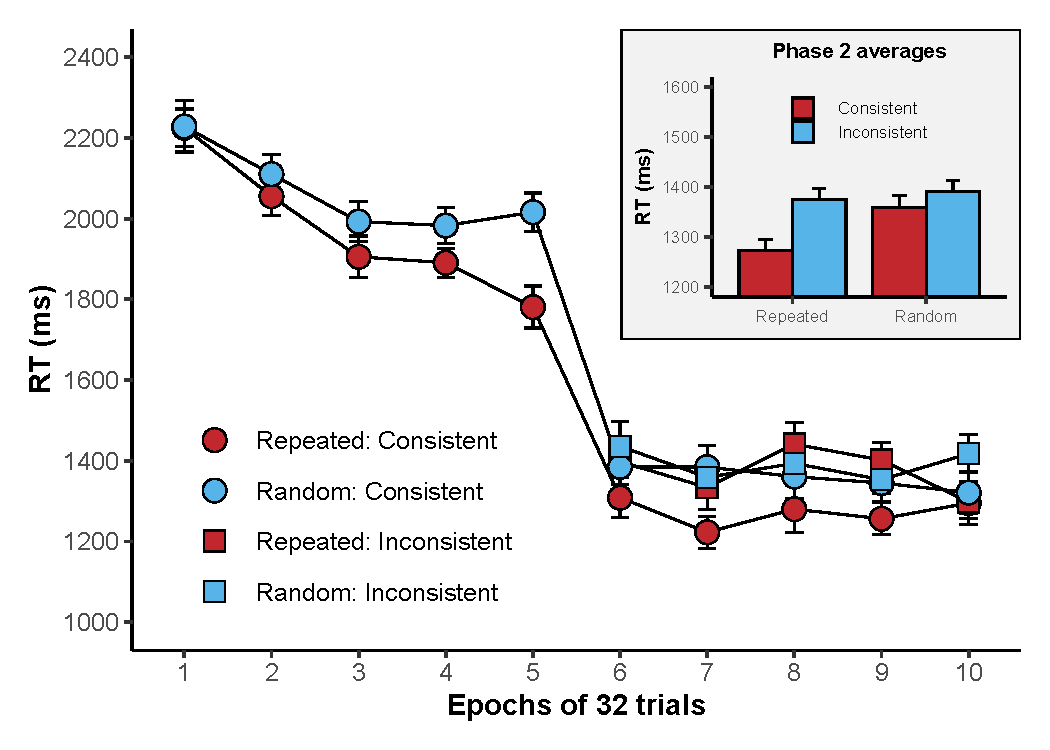
\includegraphics{CCC_ms1_files/figure-latex/Exp1-RT-figure-1} 

}

\caption{RT data for Experiment 1}\label{fig:Exp1-RT-figure}
\end{figure}

These data were explored with a Bayesian ANOVA, using the \emph{BayesFactor::anovaBF()} function (for all analyses in this study the priors were set at the default ``medium'' width). First taking the data from phase 1 (epochs 1-5), the model with the largest Bayes Factor (BF) contained the factors of epoch and configuration (repeated vs.~random), BF\textsubscript{10} = 2.2x10\^{}12. The addition of the interaction term did not substantially improve the model fit, BF\textsubscript{10} = 0.5.

A Bayesian ANOVA on the data from phase 2 (epochs 6-10) found significant support for the model containing the factor of configuration, BF\textsubscript{10} = 88.22. There was evidence to suggest that the addition of the factor of epoch did not substantially improve the model predictions, BF\textsubscript{10} 0.0. Comparing the response times from just ``repeated: consistent'' trials with their respective random trials (random: consistent), revealed support for a difference between these trial types, BF\textsubscript{10} = 4.87. There was no evidence to support a difference between the ``repeated: inconsistent'' trials and the respective random trials, BF\textsubscript{10} = 0.39. There was substantial support for a difference between the repeated consistent and the repeated inconsistent trials, BF\textsubscript{10} = 10.34.

\hypertarget{discussion}{%
\subsection{Discussion}\label{discussion}}

Experiment 1 sought to examine the consequence of an endogenous cue that prompts top-down control of the search process on contextual cuing. In phase 1 we established a robust contextual cuing effect. Following this, participants received instruction that each trial would be preceded by an arrow stimulus that would signal the side of the screen on which the target would appear. This cue was valid on all trials in phase 2. Consistent with these instructions and the processing of this cue, we observed substantially reduced search times in phase 2 compared to phase 1. The same set of repeated configurations were presented in Phase 2, but for half of the trials, the target was relocated to the diagonally opposed quadrant of the screen. Therefore, on these ``repeated inconsistent'' trials, the underlying configuration of distractors predicted the target in a location that opposed that of the (valid) endogenous cue. Across this phase we observed significant contextual cuing for the repeated consistent trials, demonstrating that the underlying configuration of distractors continues to guide attention in the presence of the endogenous cue. However, the repeated inconsistent trials did not lead to an impairment in response times relative to random trials, suggesting that the underlying configuration did not influence search on these trials.

\hypertarget{experiment-2}{%
\section{Experiment 2}\label{experiment-2}}

In Experiment 1 we demonstrated that an established effect of contextual cuing is maintained even when attention is being guided by the presence of a valid endogenous cue. That is, we examined whether the \emph{performance} component of contextual cuing is disrupted by a concurrent controlled attentional behaviour. In Experiment 2 we wanted to explore the \emph{learning} of the contextual cue itself, examining whether the presence of a valid endogenous cue may limit the development of a contextual cuing effect. To do this, we trained each participant on two sets of repeating configurations. One of these sets was always presented in the presence of a valid endognenous cue, while the other set was always presented in the absence of the endogenous cue. The extent to which there is a ``cue-competition'' effect between the endogneous cue and the contextual cues can be examined by comparing the contextual cuing effect we observe for the two sets of configurations. Given the (expected) difference in RTs we observed in Experiment 1, between the trials with the endogenous cue present and the cue being absent, in a second phase of Experiment 2 we removed the endogenous cue entirely from the task. This second phase therefore allowed us to directly compare the contextual cuing for the two sets of participants when RTs are of the same magnitude.

``Cue-competition'' effects have been examined previously in contextual cuing. Endo and Takeda (2004) trained participants with a contextual cuing task composed of distractor location configurations and repeating distractor identities. Their experiments suggested that the stronger configural (spatial) cue out-competed the cue provided by the distractor identities. Similarly, Kunar et al. (2014) found that when colour cues and configural cues both predicted the target location, configural cues were dominant and tended to overshadow the weaker colour cue. T. Beesley and Shanks (2012) looked at the cue-interaction effects \emph{within} a configuration of distractors. Participants were first trained with half a configuration of repeating distractors that predicted the target (8 out of 16 distractors). In a later stage these distractors were paired with a new half-configuration, such that the whole configuration now predicted the same target location. In contrast to the predictions of the vast majority of models of contingency learning, learning about these new predictive distractors was facilitated, rather than impaired in this second phase (relative to a control condition). Thus, T. Beesley and Shanks (2012) found that cue-competition was not observed within a configuration of equally predictive distractors. Together these studies suggest that the repeated configuration will out-compete non-configural cues for access to the learning mechanism. The dominance of the configuration in these situations may therefore lead to the prediction that the endogenous cue would not ``block'' the learning of the configuration in this task.

\hypertarget{method-1}{%
\subsection{Method}\label{method-1}}

\hypertarget{participants-1}{%
\subsubsection{Participants}\label{participants-1}}

Thirty-one undergraduate students from Lancaster University were recruited (mean age = 20.13, SD = 1.09; 17 identified as male and 14 as female) via the Psychology Research Participation System in the Department of Psychology at Lancaster University, in return for the opportunity to use the recruitment system for their own research in future years.

\hypertarget{materials-1}{%
\subsubsection{Materials}\label{materials-1}}

The materials and stimuli were identical to Experiment 1.

\hypertarget{design-1}{%
\subsubsection{Design}\label{design-1}}

Four repeated configurations were created in an identical manner to those used in Experiment 1. For each participant, two of these configurations were used for the ``cue-competition'' condition, in which the arrow cue was presented before the configuration, while two were used for the ``control'' condition (no arrow presented). As in Experiment 1, the four repeated configurations were paired with unique target positions from each of the four quadrants. We counterbalanced the use of the target quadrants across the factors of configuration type (repeated and random) and cue condition (cue-competition and control). For half of the participants, targets in the top left and bottom right were used for the repeated configurations presented with the arrow (cue-competition) condition, with targets in the top right and bottom left used for repeated configurations in the no-arrow (control) condition. For these participants, random configurations presented with the arrow had targets in the top right and bottom left, and random configurations without the arrow had targets in the top left and bottom right. For the other half of the participants these assignments were revered (repeated-arrow: top-right and bottom-left; repeated-no arrow: top-left and bottom-right; random-arrow: top-left and bottom-right; random-no arrow: top-right and bottom-left).

\hypertarget{procedure-1}{%
\subsubsection{Procedure}\label{procedure-1}}

The procedure was the same as Experiment 1 with the following differences. Participants received 320 trials in total. For the first 160 trials, the arrow was presented for the relevant conditions. For the final 160 trials, the arrow was never presented. Rest breaks were given every 60 trials.

\hypertarget{results-1}{%
\subsection{Results}\label{results-1}}

Our criteria for removing outlier data were identical to Experiment 1. On average, trials ended with a timeout on 2.13\% of trials (SD = 1.83). Zero participants had an usually high proportion of timeouts. The mean accuracy of participants (not including timeout trials) was 95.85\% (SD = 6.10\%). One participant had an unusually low proportion of accurate trials and were also removed. Zero participants were deemed to be an outlier in terms of mean RT.

For the remaining thirty-three participants we removed trials with a timeout and inaccurate trials, before removing outliers from the RT data. On average, the proportion of outliers removed was 2.81\% (SD = 1.04\%). One participant had an unusual proportion of trials removed as outlier RTs and were not included in the final analysis.

\begin{figure}

{\centering 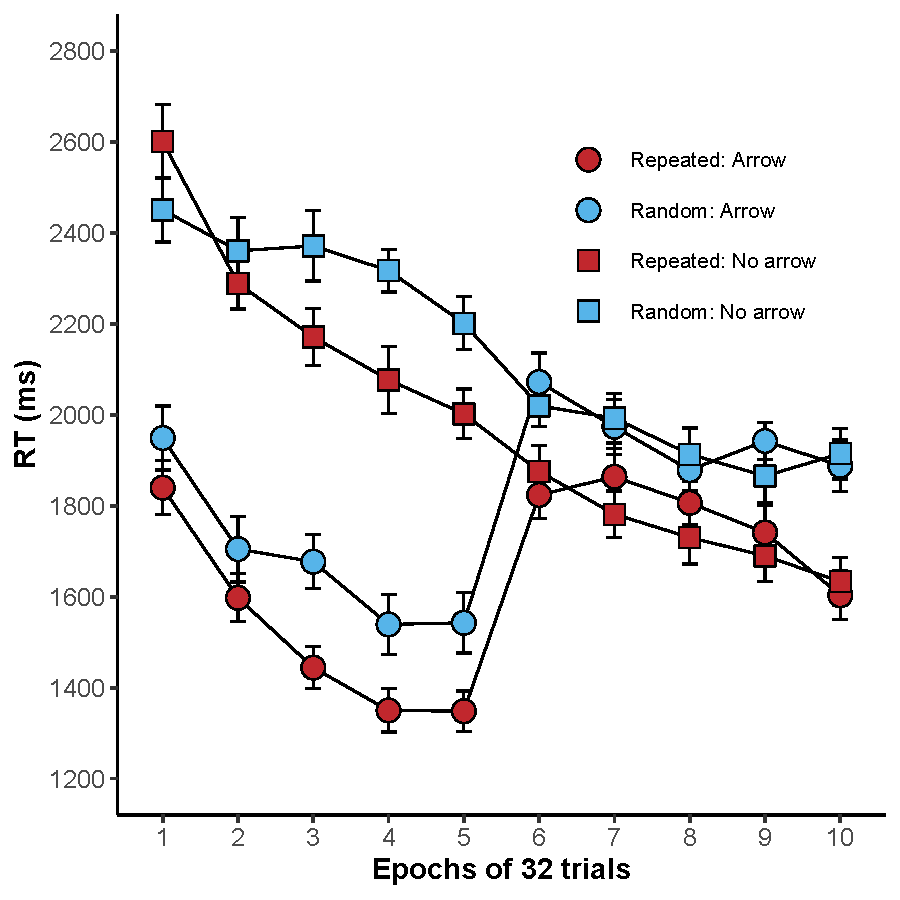
\includegraphics{CCC_ms1_files/figure-latex/Exp2-RT-figure-1} 

}

\caption{RT data for Experiment 2}\label{fig:Exp2-RT-figure}
\end{figure}



Figure \ref{fig:Exp2-RT-figure} shows the RT data across the 10 epochs of the experiment. Contextual cuing emerged rapidly in both the arrow and no-arrow conditions, with little suggestion that the CC effect was different in the two cuing conditions. The Phase 1 data were explored with a Bayesian ANOVA, which revealed that the the model with the largest Bayes Factor (BF) contained the factors of epoch, configuration (repeated vs.~random), endogenous cue (arrow present vs.~arrow absent), and the interaction of epoch and configuration, BF\textsubscript{10} = 6.8x10\^{}37. The addition of the interaction term between endongenous cue and configuration did not improve the fit of the model, BF\textsubscript{01} 0.44.

It is noteworthy that in epoch 1 of the no-arrow condition, participants responded more slowly to repeated configurations than random configurations, a result that almost certainly reflects noise in the data, and not a systematic effect of the configuration type. Indeed, this slower acquisition of the contextual cuing effect in this condition was the opposite of what we predicted on the basis of the competition hypothesis. An exploratory analysis examining the data from epochs 2 to 5 revealed greatest support for the model that contained the three factors, but no interaction effects between them, BF\textsubscript{10} = 2.5x10\^{}37. In this analysis there was support for an absence of an interaction between the factors of configuration and endogenous cue, BF\textsubscript{01} 0.18 ± 4.67\%.

BF\textsubscript{01} =3x10\^{}22±0.84\%

When the endogenous cue was removed in the second half of the experiment, RTs were equivalent across the two conditions. An effect of configuration was seen for both cuing conditions, with little discernible difference between the size of the cuing effects. We conducted a Bayesian ANOVA with factors of epoch, configuration and endogenous cue condition (arrow vs.~no-arrow). The best fitting model was that with just the factors of epoch and configuration with no interaction between the factors, BF\textsubscript{10} =6.5x10\^{}9 ± 2.28\%. To examine the evidence in support of the interaction of the configuration and endongenous cue factors, we compared the model containing the three factors to the model containing the three factors plus the interaction of configuration and endogenous cue, which revealed support for the absence of an interaction, BF\textsubscript{01} = 0.23 ± 4.86\%.

To provide further support for the absence of the interaction between the factors of configuration type and endogenous cue, the data from across the experiment (epochs 1-10) were analysed with a Bayesian ANOVA with only the factors of configuration and endogenous cue. The best fitting model was that with the two factors and no interaction, BF\textsubscript{10} =3.6x10\^{}5 ± 2.69\%. The addition of the interaction term did not strengthen the model, with support evident for the absence of the interaction, BF\textsubscript{01} = 0.33 ± 5.35\%.

\hypertarget{discussion-1}{%
\subsection{Discussion}\label{discussion-1}}

Experiment 2 sought to examine whether the presence of a valid endogenous cue would compete for the acquisition of a contextual cuing effect. In the first phase, two sets of configurations were trained, one of which was always presented in the presence of the endogenous cue, and one set which was presented without the cue. Overall there was considerable evidence that the cue was processed and acted upon, as respones times to the target were much faster on cued trials. However, there was no evidence to suggest that this impaired the acquisition of the configurations on those trials. Similarly, when the endogenous cue was never presented in the final phase of the experiment, the level of contextual cuing was also equivalent between the two sets of configurations. The Bayesian analyses found support for the equivalence of these CC effects.

The lack of competition effects seen in Experiment 2 are at odds with some findings in the CC literature (i.e., (Endo \& Takeda, 2004; Kunar et al., 2014)), where competition has been seen by more dominant or salient features of the displays. Instead, the findings point towards a more automatic nature to contextual cuing, whereby associations form ubiquitously, so long as they can recieve the focus of attention at some point within the search process (e.g., T. Beesley and Shanks (2012))

\hypertarget{experiment-3}{%
\section{Experiment 3}\label{experiment-3}}

Experiment 3 sought to examine \ldots{}

\hypertarget{method-2}{%
\subsection{Method}\label{method-2}}

\hypertarget{participants-2}{%
\subsubsection{Participants}\label{participants-2}}

Forty-three undergraduate students from Lancaster University were recruited (mean age = 18.65, SD = 2.81; 29 identified as male and 12 as female) via the Psychology Research Participation System in the Department of Psychology at Lancaster University, in return for the opportunity to use the recruitment system for their own research in future years.

\hypertarget{materials-2}{%
\subsubsection{Materials}\label{materials-2}}

The materials and stimuli were identical to Experiment 1.

\hypertarget{design-2}{%
\subsubsection{Design}\label{design-2}}

\hypertarget{procedure-2}{%
\subsubsection{Procedure}\label{procedure-2}}

\hypertarget{results-2}{%
\subsection{Results}\label{results-2}}

Our criteria for removing outlier data were identical to Experiment 1. On average, trials ended with a timeout on 3.33\% of trials (SD = 4.08). One participants had an usually high proportion of timeouts. The mean accuracy of participants (not including timeout trials) was 96.12\% (SD = 8.47\%). Two participants that had an unusually low proportion of accurate trials and were also removed. Zero participants were deemed to be an outlier in terms of mean RT.

For the remaining forty participants we removed trials with a timeout and inaccurate trials, before removing outliers from the RT data. On average, the proportion of outliers removed was 3.13\% (SD = 0.72\%). zero participants had an unusual proportion of trials removed as outlier RTs and were not included in the final analysis {[}EAF4S{]}.

\begin{figure}

{\centering 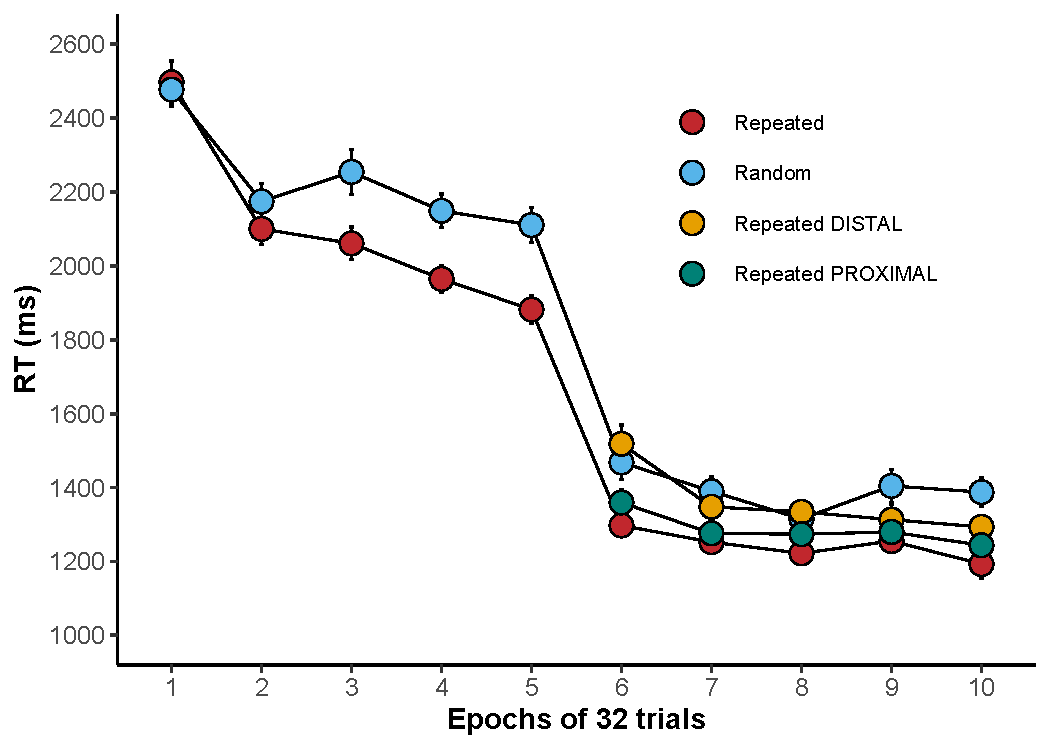
\includegraphics{CCC_ms1_files/figure-latex/Exp3-RT-figure-1} 

}

\caption{(ref:Exp3-RT-figure)}\label{fig:Exp3-RT-figure}
\end{figure}

\newpage

\hypertarget{references}{%
\section*{References}\label{references}}
\addcontentsline{toc}{section}{References}

\hypertarget{refs}{}
\begin{CSLReferences}{1}{0}
\leavevmode\vadjust pre{\hypertarget{ref-beesley2012}{}}%
Beesley, T., \& Shanks, D. R. (2012). Investigating cue competition in contextual cuing of visual search. \emph{Journal of Experimental Psychology: Learning, Memory, and Cognition}, \emph{38}(3), 709--725. \url{https://doi.org/10.1037/a0024885}

\leavevmode\vadjust pre{\hypertarget{ref-beesley2015b}{}}%
Beesley, Tom, Vadillo, M. A., Pearson, D., \& Shanks, D. R. (2015). Pre-exposure of repeated search configurations facilitates subsequent contextual cuing of visual search. \emph{Journal of Experimental Psychology: Learning, Memory, and Cognition}, \emph{41}(2), 348--362. \url{https://doi.org/10.1037/xlm0000033}

\leavevmode\vadjust pre{\hypertarget{ref-cousineau2005}{}}%
Cousineau, D. (2005). Confidence intervals in within-subject designs: {A} simpler solution to {Loftus} and {Masson}'s method. \emph{Tutorials in Quantitative Methods for Psychology}, \emph{1}(1), 42--45. \url{https://doi.org/10.20982/tqmp.01.1.p042}

\leavevmode\vadjust pre{\hypertarget{ref-endo2004}{}}%
Endo, N., \& Takeda, Y. (2004). Selective learning of spatial configuration and object identity in visual search. \emph{Perception \& Psychophysics}, \emph{66}(2), 293--302. \url{https://doi.org/10.3758/BF03194880}

\leavevmode\vadjust pre{\hypertarget{ref-kunar2014}{}}%
Kunar, M. A., John, R., \& Sweetman, H. (2014). A configural dominant account of contextual cueing: {Configural} cues are stronger than colour cues. \emph{Quarterly Journal of Experimental Psychology (2006)}, \emph{67}(7), 1366--1382. \url{https://doi.org/10.1080/17470218.2013.863373}

\end{CSLReferences}


\end{document}
